\chapter{Classificação de dispositivos}

Num ambiente em que dispositivos podem se movimentar livremente e cujos serviços devem ser compartilhados de forma transparente ao usuário, torna-se necessário que cada dispositivo presente na rede possa se comunicar facilmente com os demais, independente de quais tecnologias, padrões ou protocolos tenham sido adotados. É fundamental que essa comunicação seja feita de forma tão rápida e confiável quanto possível, pois toda atividade do \emph{middleware} com seus clientes depende dela, inclusive o processo de classificação dos recursos disponíveis no \emph{smart space}, ideia central deste documento.

\section{Formas de classificação}

Existem duas formas principais de realizar a classificação de dispositivos pretendida:

\begin{itemize}
	\item Fixa:
		Conjunto fixo de classificações não relacionadas.
	\item Relacionada:
		Estabelece relações entre os tipos básicos pré-definidos e suas especializações.

\end{itemize}

As classificações de forma Relacionada possuem a vantagem de reutilizar atributos definidos em outras classes e de poder adicionar novos atributos especializando os tipos relacionados, o que evita redundância na definição das classes. Enquanto as classificações de forma Fixa possuem a vantagem de serem mais simples de serem definidas.

Uma importante propriedade de uma classificação é a hierarquia, ou seja, uma representação em que as categorias da classificação podem ser especializadas formando novas categorias mais específicas, com diferentes atributos. Existem diferentes maneiras conhecidas de se representar uma hierarquia de forma a relacionar categorias que tenham atributos em comum: arquivos no formato XML, hierarquia de classes, ontologia ou simplesmente não utilizar uma hierarquia onde as categorias não tem relações entre si, caso da forma Fixa de classificação.

O XML (\emph{Extensible Markup Language}), como seu próprio nome sugere, pode ser estendido e dessa forma, é possível montar uma hierarquia de arquivos XML. O seu uso para descrever um tipo de dispositivo tem a vantagem de ser independente de plataformas de hardware ou software e, devido sua formatação, possui uma boa legibilidade, não necessitando de um pré-processamento por parte de um computador para seu conteúdo se tornar compreensível. Esse formato possui, contudo, a desvantagem de repetir uma grande quantidade de informação o que pode prejudicar a velocidade de comunicação entre dispositivos que o utilizem. Outro fator que deve ser levado em consideração é que o conjunto de protocolos \emph{uP} (\emph{Ubiquitous Protocols}) do \emph{middleware} \emph{uOS} utiliza o formato JSON para troca de mensagens, um mecanismo mais leve, e ainda assim estruturado, para representar informação.

A Hierarquia de Classes é amplamente utilizada em Programação Orientada à Objetos. Uma classe possui atributos ou propriedades e uma outra classe pode herdar esses atributos e criar uma especialização dessa classe raiz, à esse relacionamento dá-se o nome de Herança. Dependendo da linguagem orientada utilizada, uma Classe pode herdar métodos e atributos de várias outras Classes, formando uma herança múltipla de classes, ou então poderá cada Subclasse poderá herdar de apenas uma outra Classe, não podendo, entretanto, ocorrer uma herança circular, onde uma Classe A herda de uma Classe B, que por sua vez herda atributos de uma Classe C que especializa a Classe A. Uma Hierarquia de Classes forma, portanto, uma espécie de árvore de classes.

Ontologia é uma descrição formal de conceitos (classes) em um determinado domínio. Esses conceitos possuem propriedades, que descrevem atributos, características e restrições. De forma semelhante à orientação à objetos, conceitos podem possuir subclasses que especializam a classe superior. A Ontologia já permite uma herança múltipla de classes, e novos conceitos podem ser construídos por meio do relacionamento entre classes. Para construir uma Ontologia deve-se definir as classes do domínio, distribuir as classes de forma hierárquica, definir valores e restrições para suas propriedades e utilizar esses valores nas instâncias das classes da Ontologia. 

\begin{comment}
Dessa forma, temos uma base de conhecimento. As Ontologias se tornaram populares na Web por dividir produtos em categorias e em características em sites de venda, e atualmente são utilizadas para compartilhar informação entre pessoas e agentes inteligentes. Uma antologia provê reutilização de conhecimento e torna explícitas as hipóteses sobre um domínio e análise do domínio.
\end{comment}


\section{Padrões}
%Apresentar os padrões. Focar nas classificações feitas por eles, pontos fortes e fracos.

Nesta seção, discutir-se-á cinco dos principais protocolos e/ou padrões pesquisados que fazem uso de uma classificação de recursos e utilizam as estratégias supracitadas para representar sua hierarquia de recursos: UPnP, IEEE 1451, DLNA, USB e \emph{Bluetooth}.

\subsection{UPnP}
O \emph{Universal Plug and Play Protocol}(UPnP) é uma arquitetura para conectividade entre aplicações inteligentes, em execução em computadores e dispositivos \emph{wireless} em geral. Ela foi definida para facilitar a conectividade entre dispositivos em diferentes ambientes, como casas, pequenas empresas ou espaços públicos~\cite{upnpArch}. A arquitetura foi desenvolvida de forma a não necessitar de configurações e fornecer uma rede invisível com descoberta automática de dispositivos de diferentes fabricantes e diversas categorias. Dessa maneira, quando um novo dispositivo entra nessa rede, ele é identificado por um IP, publica seus serviços e conhece os serviços de outros dispositivos do ambiente. 

O UPnP utiliza o nome "Universal", pois não é necessária a utilização de ~\emph{drivers} para cada dispositivo. Para atingir esse objetivo, essa arquitetura faz uso de protocolos de internet bem conhecidos como IP, TCP, UDP, HTTP, além do formato XML, para facilitar a interoperabilidade entre dispositivos diversos. Da mesma forma que os protocolos de internet, os contratos dos serviços dos dispositivos são escritos em XML e enviados por HTTP.

Após a entrada do dispositivo em uma rede, ele recebe um IP via DHCP ou gera um IP para si, no caso de redes não gerenciadas. A \emph{UPnP Device Architecture}(UDA) divide os dispositivos em duas categorias principais: dispositivos controlados ou simplesmente "dispositivos" e pontos de controle~\cite{upnpArch} formando uma espécie de arquitetura cliente(pontos de controle)-servidor(dispositivos). 

\begin{comment}	
Quando um dispositivo entra na rede UPnP, ele comunica seus serviços para os pontos de controle ou, caso seja um ponto de controle, o protocolo de descoberta do UPnP permite que ele procure dispositivos de seu interesse. O segundo passo é o envio da descrição detalhada do dispositivo para os pontos de controle, que de posse dessa descrição podem enviar mensagens de controle para o dispositivo(passo 3). Os pontos de controle podem também assinar um contrato para envio de notificações de evento utilizando algum dos serviços que o dispositivo provê(passo 4). O último passo é de apresentação. Caso o dispositivo possua uma URL de apresentação é possível abrir uma página \emph{web} no \emph{browser} e um usuário pode controlar o dispositivo por meio dessa página~\cite{upnpArch}.
\end{comment}


Nosso foco neste trabalho se encontra no segundo passo do processo: a descrição dos dispositivos. Após sua descoberta, os pontos de controle ainda não têm muita informação sobre o dispositivo, então os pontos de controle interessados solicitam a descrição do dispositivo via uma URL que este dispositivo disponibilizou durante primeira etapa.

A descrição de um dispositivo definida no UPnP é feita por meio de um arquivo XML que inclui informações sobre o fabricante, lista de dispositivos embarcados ou serviços e para cada serviço, URLs para controle, eventos e apresentação. A descrição de serviços inclui ainda uma lista de comandos ou ações que o dispositivo deverá responder e para cada ação existem parâmetros ou argumentos. O estado do serviço é representado por uma lista de variáveis.

O UPnP define uma série de classificações pré-determinadas que os fabricantes podem utilizar na definição de seus dispositivos. Um característica encontrada nessas classificações é a sua leveza de serem implementadas por dispositivos com pouca capacidade de computação, embora também possam ser utilizadas por dispositivos mais robustos como computadores. São elas:

\begin{itemize}
\item Áudio/Vídeo:
	Essa categoria possui duas principais sub-classificações que foram sendo atualizadas com o desenvolvimento de novas tecnologias: 
	\begin{itemize}
		\item \emph{Media Server}:

			Define um dispositivo genérico que provê conteúdo de áudio e/ou vídeo, como CD e DVD \emph{players}, cameras, rádios, televisões e \emph{set-top boxes}. Embora, seja utilizado por dispositivos com diferentes capacidades de processamento e conteúdos, o \emph{Media Server} expõe conteúdo de forma consistente.

		\item \emph{Media Renderer}:

			Define um dispositivo genérico capazes de renderizar conteúdos de áudio e/ou vídeo como MP3 \emph{players} e televisões. Dependendo da implementação de um \emph{Media Renderer}, pode-se utilizar os recursos de auto-falante de uma televisão para consumir um serviço de música de um \emph{Media Server}.
	\end{itemize}
\item Gerenciamento de Dispositivos:
	Essa categoria foi criada para adicionar operações gerenciais à qualquer dispositivo UPnP. Esse gerência inclui funções para configuração de serviços e do próprio dispositivo, diagnóstico e correção de problemas além de gerência do \emph{firmware} e dos \emph{softwares} do dispositivo.

\item Automação Residencial:
	\begin{itemize}
		\item Cortina de Proteção Solar:

			Provê uma sombra por meio de uma cortina. Seu controle pode ser manual, automático ou desabilitado. Sua especificação não contempla configurações a respeito da automação da cortina ou proteções.
		\item Câmera Digital de Segurança:

			Provê controle básico sobre a configuração da câmera, contendo serviços de fotos e vídeos.
		\item Aquecimento, Ventilação e Ar Condicionado:
			
			Esse dispositivo conta com auxílio de sensores de temperatura e possui a capacidade de saber ou controlar a temperatura do ambiente por meio de ventiladores e ar-condicionados.
		\item Controles de Luz:
			
			São divididos em Luz binária, que representa uma lâmpada ou qualquer dispositivo emissor de luz que possa somente estar apagado ou aceso, e em Luz cuja intensidade pode ser alterada, 
	\end{itemize}

\item Rede:
	\begin{itemize}
		\item \emph{Gateway} de Internet:
			
			Essa classificação define um dispositivo de interconexão entre uma rede residencial local (LAN) e a \emph{Wide Area Network} (WAN), provendo conectividade com a internet.
			\begin{itemize}
				\item Dispositivo de Conexão WAN: É um dispositivo virtual definido tendo o \emph{Gateway} de Internet como raiz. Funciona como um contêiner para um \emph{link} ou serviços de conexão em uma interface WAN. 
				\item Dispositivo WAN: É um dispositivo virtual efinido tendo o \emph{gateway} de internet como raiz. Cada dispositivo WAN é uma instância virtual de uma interface WAN no \emph{gateway} de internet. Múltiplas interfaces físicas WAN para clientes UPnP, existirão distintas instâncias deste dispositivo.
			\end{itemize}

		\item Ponto de acesso WLAN(\emph{Wireless Local Area Netowork}):
			
			Esse dispositivo implementa os padrões IEEE 802.11 (a,b,g) sem fio para prover uma infraestrutura de rede para casas e pequenas empresas. Essa definição não inclui uso dos pontos de acesso como \emph{hotspots} ou redes de grandes empreendimentos. O ponto de acesso age com uma ponte \emph{Ethernet} que permite ligações de múltiplos nós com a LAN.
	\end{itemize}

\item Impressora:
	Define um dispositivo com capacidade de impressão. Essa especificação não abrange dispositivos que possuem funções de FAX ou \emph{Scanner}, que possui uma especificação própria.

\item Acesso Remoto:
	Essa categoria é dividida entre dois dispositivos:
	\begin{itemize}
		\item Agente de Descoberta de Acesso Remoto:

			Possui a função de prover a capacidade de sincronizar a informação sobre a descoberta UPnP entre duas redes remotas.
		
		\item Servidor de Acesso Remoto:
		
			Permite que pontos de controle configurem Servidores de Acesso Remoto.

	\end{itemize}

\item Interface Remota:
	Classifica dispositivos entre servidores e clientes de uma interface remota com o usuário.

\item \emph{Scanner}:
	Representa um dispositivo de \emph{Scanner} com \emph{feeder} opcional. Esse dispositivo possui os serviços de digitalização via \emph{feeder} ou \emph{flatbed} e um serviço para configuração com o painel frontal do dispositivo. Essa categoria não contempla funcionalidades de Fax ou cópias.

\item Telefonia:
	\begin{itemize}
		\item Servidor de Telefonia:

			Permite que pontos de controle gerenciem chamadas telefônicas, mensagens e presença por meio de outros dispositivos UPnP. 

		\item Cliente de Telefonia:
		
			Permite que pontos de controle possam gerenciar mídias por meio de um de um servidor de telefonia.
				
	\end{itemize}

\item Básico:
	A definição de dispositivos básicos provêm um mecanismo para produtos que não se enquadram em uma classificação adequada do UPnP, possam utilizá-lo. Por esse motivo, essa especificação não possui nenhum serviço definido, mas pode ser utilizada como dispositivo raiz para outras categorias já definidas.
\end{itemize}

Os fabricantes podem, a partir de uma classificação padrão, estender e especializar determinada definição adicionando novos serviços, por exemplo, o que sugere uma hierarquia de dispositivos por meio de arquivos XML. Um fator interessante nas classificações de dispositivos UPnP é que sua especificação já traz consigo a especificação de serviços que esses dispositivos provêm. 

\subsection{IEEE 1451}
O IEEE 1451 se divide em uma família de padrões que foram criados com os objetivos de permitir a capacidade de comunicação entre transdutores(sensores e atuadores) de forma \emph{plug-and-play} por meio de redes com ou sem fio, facilitar a criação de transdutores com inteligência embarcada, simplificar a configuração e manutenção de sistemas, prover comunicação entre transdutores legados, e por fim, habilitar a implementação de transdutores inteligentes e com uso mínimo de memória~\cite{ieee1451journal}.

Um dos padrões da família, o IEEE 1451.1, define um modelo de informação para \emph{Network Capable Application Processors} (NCAP) que foi estabelecido para especificar um modelo de objetos comum e interfaces de componentes da rede de transdutores. Dessa forma, foi desenvolvido um \emph{framework} orientado a objetos que pode ser estendido para facilitar o desenvolvimento de aplicações que foi definido da seguinte forma: Um modelo de dados que especifica a forma e o tipo de comunicação, tanto local quanto remota, por meio das interfaces de objetos 1451.1, um modelo de objetos que especifica tipos de componentes de software usados para definir e implementar sistemas e, por fim, modelos de comunicação que definem a sintaxe e semântica das interfaces de software entre redes de comunicação e objetos de aplicação~\cite{ieeeOO1451}~\cite{ieee1451monitoring}.

\begin{figure}[ht]
\center
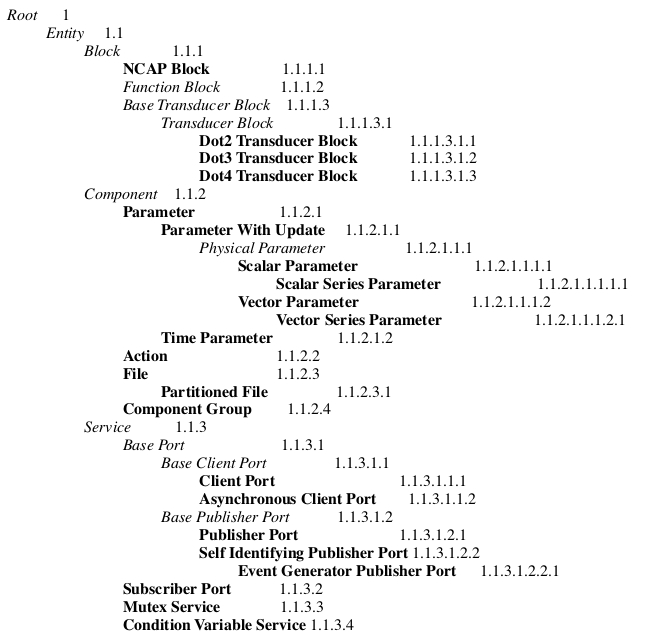
\includegraphics[scale=0.5]{imagens/ieee1451-classHierarchy}
\caption{Hierarquia de Classes do Padrão IEEE 1451.1}
\label{fig:classHierarchy}
\end{figure}

O padrão ~\cite{ieee1451standard} especifica cada classe no modelo definindo as interfaces da classe(por meio de assinaturas e operações) e o comportamento da classe (via texto ou máquinas de estado). A figura~\ref{fig:classHierarchy} mostra a hierarquia de classes definida pelo padrão em que as classes em itálico representam classes abstratas. Nesta figura é possível observar 3 tipos principais de objetos IEEE 1451.1:

\begin{itemize}
	\item\emph{Block}:

	Especializada em três classes:
		\begin{itemize}
			\item\emph{NCAPBlock}:
				Provê interfaces para comunicações de rede e configurações do sistema.
			\item\emph{BaseTransducerBlock}:
				Provê interfaces entre transdutores e funções.
			\item\emph{FunctionBlock}:
				Provê encapsulamento de funções específicas.
		\end{itemize}
	
	\item\emph{Component}:
	
		Fornecem:
		\begin{itemize}
			\item Informações estruturadas: medidas e arquivos.
			\item Coleções de objetos relacionados com a aplicação.
			\item Ações com estados onde a ação é executada após um período de tempo.
		\end{itemize}
	\item\emph{Service}:
	
		Suportam:
		\begin{itemize}
			\item Comunicação entre objetos de diferentes NCAPs.
			\item Sincronização do sistema.
		\end{itemize}
\end{itemize}

Há ainda as classes não-IEEE 1451.1, que não estão representadas na Figura ~\ref{fig:classHierarchy} e possuem restrições de aplicabilidade na arquitetura IEEE 1451.



\subsection{DLNA}

A \emph{Digital Living Network Alliance} (DLNA) é uma organização composta pelas principais empresas de eletrônicos de consumo, computação e dispositivos móveis. Foi fundada em 2003 e tem como objetivo fornecer orientações para permitir a interoperabilidade entre dispositivos para completar a convergência da indústria digital, levando, dessa forma, inovação, simplicidade e valor para os consumidores~\cite{dlnaoverview}. Tem como visão facilitar a criação, o gerenciamento e o compartilhamento de conteúdo digital (fotos, músicas e vídeos) entre os dispositivos pertencentes à mesma rede~\cite{dlnahdvideostreaming}. Deve permitir, por exemplo~\cite{dlnaoverview}:

\begin{itemize}
	\item Facilmente adquirir, armazenar e acessar música digital a partir de praticamente qualquer lugar da casa;
	\item Facilmente gerenciar, visualizar, imprimir e compartilhar fotos digitais;
	\item Transportar seu conteúdo favorito a partir qualquer lugar, mesmo que as pontas envolvidas estejam em movimento;
	\item Aproveitar a gravação e reprodução de conteúdo distribuído e multi-usuário.
\end{itemize}

Imagine, por exemplo, uma situação hipotética em que uma pessoa deseja compartilhar um pequeno vídeo com seus amigos a partir de seu celular. A fim de exibir esse vídeo em sua TV widescreen na sua sala de estar, ela necessita, primeiramente, envia-lo para seu próprio email. Em seguida, deve ligar seu PC, fazer o download do vídeo e salvá-lo em um \emph{pendrive} ou cartão de memória. Posteriormente, deve ligá-lo na TV ou em um receptor digital e, então, utilizar a interface do dispositivo para localizar o vídeo e exibi-lo~\cite{dlnahdvideostreaming}.

\begin{figure}[ht]
	\center
	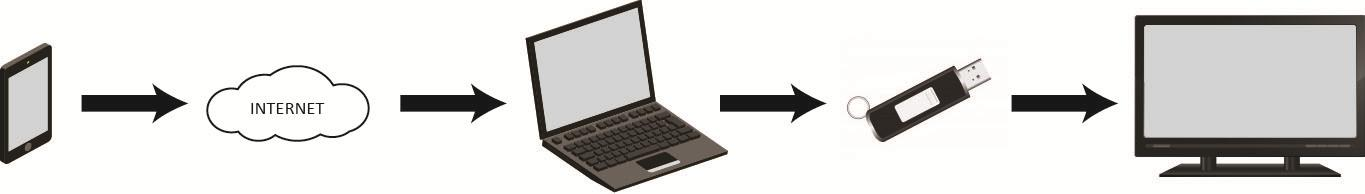
\includegraphics[scale=0.3]{imagens/dlna1}
	\caption{A exibição de um vídeo ou foto de um celular em uma TV envolve tal processo tradicional, tedioso e demorado que os consumidores raramente farão.}
	\label{fig:traditionalProccess}
\end{figure}

Além de interromper a conversa, esse tipo de processo de tranferência de conteúdo simplesmente consome muito tempo, mesmo quando ocorre sem problemas. Como resultado, a partilha informal de vídeo em múltiplas telas não é visto muitas vezes como uma opção razoável~\cite{dlnahdvideostreaming}.

Este é o valor da proposição que o DLNA oferece aos seus consumidores: a partilha contínua e sem esforço de conteúdo digital. Produtos projetados seguindo as diretrizes DLNA estabelecidas para compartilhar vídeo em apenas um único passo: a transmissão de uma cópia do vídeo do telefone sem fio para a TV. O consumidor pode até mesmo congelar o vídeo usando um "controle remoto" do menu no telefone, bem como \emph{fast-forward} e reproduzir o vídeo~\cite{dlnahdvideostreaming}.

\begin{figure}[ht]
	\center
	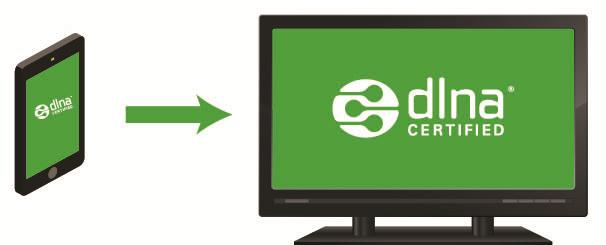
\includegraphics[scale=0.3]{imagens/dlna2}
	\caption{O valor da proposição do DLNA é o compartilhamento transparente e fácil de conteúdo, permitindo que os consumidores enviem uma cópia de um vídeo ou fotos diretamente para a TV em uma única etapa.}
	\label{fig:dlnaProccess}
\end{figure}

Suas diretrizes destacam casos de uso cuidadosamente construídos para redes domésticas (veja a tabela~\ref{tab:casosdeuso_dlna}), funções adicionais que aumentam a experiência do compartilhamento de conteúdo e doze classes de dispositivos espalhados na categoria "Rede Doméstica e Dispositivos Móveis". A classificação de um dispositivo é feita de tal forma que um único aparelho multifuncional pode possuir diversas categorias diferentes~\cite{dlnahdvideostreaming}.

Em suma, o DLNA pode ser visto como uma coleção de padrões abertos que definem como uma rede residencial interage em todos os seus níveis, ou seja, além de definir como os diferentes padrões irão interoperar e como os dados serão tratados em cada nível, ele também reduz o número de padrões que um dispositivo deve suportar.

\begin{table}
	\begin{center}
		\begin{tabular}{rl}
		\hline
		\textbf{Casos de Uso} & \textbf{Exemplo}																\\
		\hline
		Enviar & Tranferir vídeos ou imagens capturadas em uma câmera digital ou celular para um computador.	\\
		\hline
		Empurrar & Exibir vídeos ou imagens capturadas em uma câmera digital ou celular diretamente em uma TV sem intermédio de um computador. \\
		\hline
		Localizar e Reproduzir ou "Reproduzir em..."" & Utiliza um celular para localizar uma música ou vídeo armazenados em um computador, unidade de disco externa ou um dispositivo \emph{Network-Attached Storage} (NAS) e transferi-lo, via \emph{stream} ou não, para reprodução. \\
		\hline
		Puxar e imprimir ou "Imprimir em..." & Vizualizar na TV uma foto armazenada em um servidor de mídia e imprimi-la utilizando uma impressora em rede. \\
		\hline
		\end{tabular}
	\end{center}
	\caption{Exemplos de casos de uso~\cite{dlnahdvideostreaming}.}
	\label{tab:casosdeuso_dlna}
\end{table}

\begin{table}
	\begin{center}
		\begin{tabular}{rll}
		\hline
		\textbf{Camada} & \textbf{Função definida} & \textbf{Padrões}				\\
		\hline
		Transmissão Protegida & Como um conteúdo comercial está protegido em uma rede doméstica. & DTCP/IP \\
		\hline
		Formatos de Mídia & Como um conteúdo de mídia está codificado e identificado para interoperabilidade. & MPEG2, MPEG4, AVC/H.264, LPCM, MP3, AAC LC, JPEG, XHTML-Print- \\
		\hline
		Transporte de Mídia & Como um conteúdo de mídia é transferido. & HTTP, Quality of Service \\
		\hline
		Gerência de Mídia & Como um conteúdo de mídia é identificado, gerenciado e distribuído. & UPnP AV 1.0, UPnP Print Enhanced 1.0 \\
		\hline
		Descoberta e Controle & Como dispositivos se descobrem e se controlam um ao outro. & UPnP Device Architecture 1.0 \\
		\hline
		Redes IP & \multirow{2}{*}{Como dispositivos com e sem fio fisicamente se conectam e se comunicam.} & IPv4 Protocol Suite \\
		Conectividade & & Wired: Ethernet 802.3, MoCAWireless: Wi-Fi 802.11, Wi-Fi Protected Setup \\
		\hline
		\end{tabular}
	\end{center}
	\caption{Camadas padrões DLNA~\cite{dlnahdvideostreaming}.}
	\label{tab:camadaspadroes_dlna}
\end{table}
\subsection{USB}

O \emph{Universal Serial Bus} (USB) é uma arquitetura de comunicaçao que adiciona a uma máquina hospedeira a capacidade de se interconectar a uma variedade de dispositivos. Surgiu com o intuito de sanar três das principais dificuldades enfrentadas à época de sua criação~\cite{usbspec}:

\begin{itemize}
	\item Integrar as plataformas das industrias da informática e comunicação. Para tal, a troca de informações entre esses dispositivos deveria acontecer de forma ubíqua e barata;
	\item Facilitar a reconfiguração de dispositivos de um computador, tais como teclados, mouses e joysticks;
	\item Integrar todas as interfaces existentes à época em um única que pudesse ser utilizada pela maior quantidade possível de dispositivos: telefone, fax, modem, adaptadores, secretárias eletrônicas, \emph{scanners}, PDA's, teclados, \emph{mouses}, etc.
\end{itemize}

De acordo com sua especificação, suas máquinas hospedeiras devem:

\begin{itemize}
	\item Fornecer energia aos seus periféricos;
	\item Suportar todas as velocidades definidas (SuperSpeed, Low Speed, Full Speed e High SuperSpeed);
	\item Suportar todos os tipos de fluxo de dados definidos (controle, massa, interrupção e síncrono).
\end{itemize}

Entende-se por máquina hospedeira qualquer dispositivo possuidor dos recursos necessários para realizar esta função. Por exemplo, conectar uma câmera à uma impressora faz sentido, enquanto que conectar um GPS à mesma impressora, não. Assim sendo, cada máquina hospedeira não necessita se comportar exatamente como um computador, mas apenas servir como hospedeiro a certos dispositivos convenientes~\cite{usb3spec}.

Atualmente sua velocidade de comunicação varia entre 1.5 ou 12 megabits por segundo (mbs) e seu protocolo permite configurar dispositivos durante a fase de inicialização ou quando eles são plugados em tempo de execução~\cite{hid}, deixando toda parte pesada desse processo a cargo do hospedeiro~\cite{usb3spec}. Tais dispositivos são divididos em várias classes e/ou subclasses diferentes (veja a tabela~\ref{tab:dispositivos_usb}), cada qual definindo um comportamento e protocolos comuns para dispositivos que oferecem funções similares~\cite{hid}.

Um mesmo dispositivo USB pode pertencer a uma ou múltiplas classes. Por exemplo, um celular pode utilizar atributos da classe HID, Audio e Comunicação. A partir dessas divisões será possível estabelecer uma hierarquia, a qual poderá ser usada no processo de classificação dos dispositivos presentes no smartspace.

Seguem abaixo as classes existentes juntamente com suas descrições~\cite{usbclasscodes}.

\begin{comment}
\begin{table}
	\begin{center}
		\begin{tabular}{cccc}
		\hline
		\multicolumn{4}{c}{\textbf{Classes de Dispositivos}}													\\
		\hline
		Audio					&	Comunicação				&	Interface Humana (HID)	&	Físico 				\\
		\hline
		Imagem					&	Impressora				&	Disco Rígido			&	Hub 				\\
		\hline
		\emph{Smart Card}		&	Segurança de Conteúdo	&	Vídeo					&	Saúde Pessoal 		\\
		\hline
		Diagnóstico				&	Controlador Wireless	&	Diversos				&	Aplicação Específica\\
		\hline
		Fabricante Específico	&							&							&						\\
		\hline
		\end{tabular}
	\end{center}
	\caption{Exemplos de classes de dispositivos USB~\cite{usbclasscodes}.}
	\label{tab:dispositivos_usb}
\end{table}
\end{comment}

\begin{itemize}
	\item \emph{Audio}: destina-se a todos os dispositivos ou funções embutidos em aparelhos que são usados para manipular áudio, voz e quaisquer funcionalidades relacionadas. Isso inclui tanto dados de áudio (analógico e digital) quanto a capacidade de diretamente controlar tal ambiente por meio de controles de volume e tom. Não inclui a funcionalidade para operar mecanismos de transporte que estão relacionados com a reprodução de dados de áudio, tais como mecanismos de transporte de fita ou controles de unidade de CD-ROM~\cite{usbaudioclass}.

	Exemplos de tais dispositivos incluem \emph{headsets}, \emph{headphones} and \emph{microphones}~\cite{usbbasicaudioclass}.
	\item \emph{Communications and CDC Control}: há três classes que compõem a definição de dispositivos de comunicação: a Classe de Comunicação do Dispositivo, a Classe de Interface de Comunicação e a Classe de Interface de Dados. A primeira é uma definição de nível do dispositivo e é utilizada pelo hospedeiro para identificar corretamente um dispositivo de comunicação que pode apresentar diferentes tipos de interfaces. A segunda define um mecanismo de propósito geral que pode ser utilizado para habilitar todos os tipos de serviços de comunicação sobre o Universal Serial Bus (USB). A última define um mecanismo de propósito geral para permitir a transferência em massa quando os dados não atendem aos requisitos para qualquer outra classe~\cite{usbcommunicationclass}.

	Exemplos de tais dispositivos incluem:
	\begin{itemize}
		\item Telecomunicações: modens analógicos, adaptadores de terminais ISDN, telefones digitais e telefones analógicos;
		\item Dispositivos de rede: modens ADSL, modens à cabo, adaptadores/hubs \emph{Ethernet} 10BASE-T e \emph{Ethernet} cross-over cabos.
	\end{itemize}
	\item HID (\emph{Human Interface Device}): destina-se primordialmente aos dispositivos que são usados por humanos para controlar e operacionalizar quaisquer tipos de sistemas computacionais~\cite{hid}. Mais específicamente, possui as seguintes particularidades:
	\begin{itemize}
		\item Deve ser tão compacto quanto possível para evitar desperdício de espaço no dispositivo;
		\item Permitir a aplicação de software para evitar informação desconhecida;
		\item Ser extensível e robusto;
		\item Suportar hierarquias e coleções;
		\item Ser autodescritivo para permitir aplicações de software genéricos.
	\end{itemize}

	Exemplos de tais dispositivos incluem: teclados e dispositivos apontadores, painéis de controle, controles que podem ser encontrados em dispositivos como telefones, controles remotos, jogos ou dispositivos de simulação e aparelhos que não necessitam de interação humana mas que fornecem dados de forma similar aos dipositivos da classe HID~\cite{hid}.
	\item \emph{Physical}: é vista como uma extensão da classe HID para dispostivos que requerem resposta física em "tempo real". Seu foco principal está em dispositivos táteis e na implementação de sistemas com resposta à força. Contúdo, não há exigência de que os membros desta classe gerem esse tipo de efeito~\cite{usbphysicalclass}.

	Exemplos de tais dispositivos incluem: \emph{joysticks} e plataformas de movimento.
	\item \emph{Image}: 
	\item \emph{Printer}: 
	\item \emph{Mass Storage}: 
	\item \emph{Hub}: 
	\item \emph{CDC-Data}: 
	\item \emph{Smart Card}: 
	\item \emph{Content Security}: 
	\item \emph{Video}: 
	\item \emph{Personal Healthcare}: 
	\item \emph{Diagnostic Device}: 
	\item \emph{Wireless Controller}: 
	\item \emph{Miscellaneous}: 
	\item \emph{Application Specific}: 
	\item \emph{Vendor Specific}: 
\end{itemize}

\begin{comment}
Com o sucesso do protocolo, novas categorias surgiram gradualmente como alternativas às novas tecnologias e/ou aos novos dispositivos. Seguem:

\subsubsection{\emph{SuperSpeed}}

Como efeito do avanço tecnológico, o desenvolvimento dos novos tipos de dispositivos, dos formatos de mídia e dos armazenamentos de baixo custo está convergindo. Para tal, requer largura de banda significativamente maior para manter uma experiência do usuário aceitável. E o USB 3.0 atende essa necessidade adicionando uma taxa de transferência ainda maior para suprir essa demanda. Traz melhorias significativas de desempenho ao consagrado USB padrão, mantendo-se compatível com os diversos outros dispositivos USB espalhados pelo mercado. Além de melhorar a eficiência de energia, sua taxa de transferência será até dez vezes maior que a taxa de transferência do USB \emph{Hi-Speed}~\cite{usbsuperspeed}.

\subsubsection{Wireless}



\subsubsection{Hi-Speed}



\subsubsection{On-The-Go and Embedded Host}

Dentre as diversas classes existentes, uma em especial chama a atenção: \emph{Human Interface Device} (HID). Esse tipo de classe, de forma geral, destina-se primordialmente aos dispositivos que são usados por humanos para controlar e operacionalizar quaisquer tipos de sistemas computacionais~\cite{hid}. Mais específicamente, possui as seguintes particularidades:

\begin{itemize}
	\item Deve ser tão compacto quanto possível para evitar desperdício de espaço no dispositivo;
	\item Permitir a aplicação de software para evitar informação desconhecida;
	\item Ser extensível e robusto;
	\item Suportar hierarquias e coleções;
	\item Ser autodescritivo para permitir aplicações de software genéricos.
\end{itemize}

\begin{table}
	\begin{center}
		\begin{tabular}{lr}
		\hline
		\textbf{Dispositivo} & \textbf{Exemplo Descritivo} \\
		\hline
		Teclados e dispositivos apontadores & Mouses, trackballs e joysticks \\
		Painéis de controle & Maçanetas, Interruptores, botões e alavancas \\
		Controles que podem ser encontrados \\
		em dispositivos como telefones,\\
		controles remotos, jogos ou dispositivos \\
		de simulação & Luvas virtuais, câmbios, \\
		volantes e pedais \\
		Dispositivos que não necessitam de \\
		interação humana mas que fornecem dados \\
		de forma similar aos dipositivos da \\
		classe HID & Leitores de códigos de barra, \\termômetros ou voltímetros. \\
		\hline
		\end{tabular}
	\end{center}
	\caption{Exemplos de classes de dispositivos USB.}
	\label{tab:dispositivos_USB}
\end{table}
\end{comment}
\subsection{\emph{Bluetooth}}

Destina-se a substituir os cabos de conexão de dispositivos fixos e/ou portáteis mantendo altos níveis de segurança. Sua força fundamental está na capacidade de lidar simultaneamente com dados e transmissão de voz, o que fornece aos usuários uma variedade de soluções inovadoras, tais como fones de ouvido \emph{hands-free} para chamadas de voz, impressão, fax, sincronização com PCs e telefones celulares, entre outros~\cite{bluetoothoverview}.

É uma tecnologia de comunicação de curto alcance. Suas principais características são a robustez, a baixa potência e o baixo custo. Sua especificação define uma estrutura uniforme para que uma ampla gama de dispositivos possam se conectar e se comunicar uns com os outros~\cite{bluetoothoverview}.

Sua estrutura e aceitação global permitem que qualquer dispositivo \emph{bluetooth} ativado possa se conectar a outros dispositivos \emph{bluetooth} situados em sua proximidade. Uma vez estabelecida, uma conexão \emph{bluetooth} permite que aparelhos a uma curta distância se comuniquem sem a utilização de fios, ou seja, por meio de redes ad hoc conhecidas como piconets. Estas são estabelecidas de forma dinâmica e automatica assim que um dispositivo entra ou sai do seu raio de alcance, facilitando o processo de conexão por parte do usuário~\cite{bluetoothoverview}.

Cada dispositivo em uma piconet pode pertencer a várias outras piconets e, simultaneamente, se comunicar com até sete outros dispositivos presentes em uma mesma rede~\cite{bluetoothoverview}.
\subsection{Device Description Language (DDL)}
\label{subsec:ddl}

Essa linguagem provê um esquema capaz de descrever a interface dos dispositivos e um processador da linguagem para converter DDL para pacote de serviços OSGi que separa as responsabilidades entre fabricantes de dispositivos, integradores de sistemas e programadores de aplicativos~\cite{gatorTechDDL}.

\begin{figure}[ht]
\center
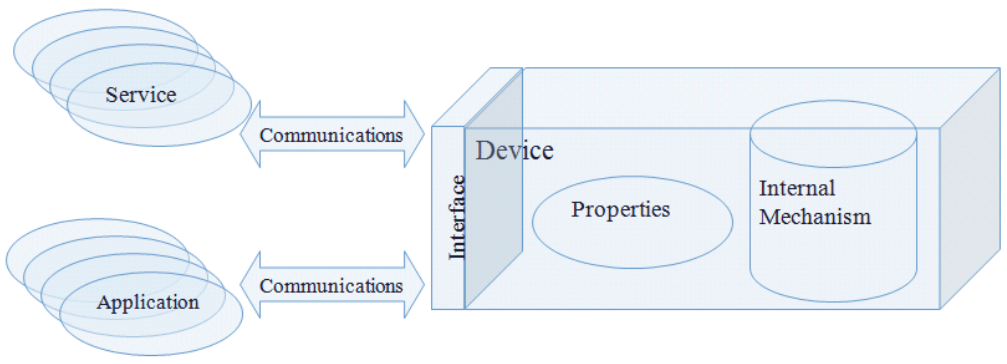
\includegraphics[scale=0.4]{imagens/gatorDDL}
\caption{Caracterização de um Dispositivo~\cite{ddlSpec}}
\label{fig:ddlspec}
\end{figure}

Na DDL, um dispositivo é caracterizado como uma entidade com propriedades, mecanismo interno e uma interface. Como mostra a figura~\ref{fig:ddlspec}. As propriedades provêem informações a respeito do dispositivo com seu propósito, suas capacidades, fabricante e requisitos operacionais. Essas informações são críticas para a integração do sistema e para programadores de serviços. O mecanismo interno é responsável pela operação do dispositivo e é desconhecido do mundo externo. A interface do dispositivo é a ponte entre o hiato entre o mecanismo interno e o mundo externo. Ela especifica a entrada e saída do dispositivo e provê um guia para aplicações e outros serviços interagirem com o dispositivo.

Os dispositivos foram classificados em três categorias:
\begin{itemize}
	\item Sensor: apenas provê dados de entrada para o usuário externo.
	\item Atuador: apenas aceita dados de saída do usuário externo.
	\item Dispositivo Complexo: provê dados de entrada e aceita dados de saída do usuário externo.
\end{itemize}

Essa classificação genérica tem a desvantagem de ser difícil de ser reutilizada e especializada por diferentes dispositivos, sendo que seus recursos são expostos na forma de serviços por meio da especificação de operações~\cite{ddlSpec}.


\section{Estado da Arte}
Nesta seção, apresentaremos alguns projetos de computação ubíqua e mostraremos como esses projetos tratam a classificação de recursos.

\subsection{Gaia}
No projeto Gaia foi criado um middleware com o objetivo de dar suporte ao desenvolvimento e execução de aplicações portáveis em \emph{Active Spaces}, ambientes com sistemas interativos, o Gaia OS, uma abstração de um sistema operacional. O middleware foi projetado para ser uma infraestrutura distribuiída que coordena entidades de software e dispositivos heterogêneos em um \emph{smart space}. O Gaia OS expõe serviços para buscar e utilizar recursos presentes no ambiente, ter conhecimento do contexto e provê um \emph{framework} para desenvolver aplicações móveis sensíveis ao contexto, que conheçam os recursos disposníveis, utilizem múltiplos dispositivos e tenham como foco o usuário~\cite{gaia2002}.

\emph{Active Spaces} são espaços físicos como escritórios, salas de conferência, casas, hospitais, campi, cidades que possuem dispositivos integrados ao ambiente. O objetivo desses dispositivos é prover e obter informação sobre usuários do ambiente, os ajudando a realizar tarefas que eles não poderiam sem os dispositivos, ou facilitando tarefas do cotidiano.

\begin{figure}[ht]
\center
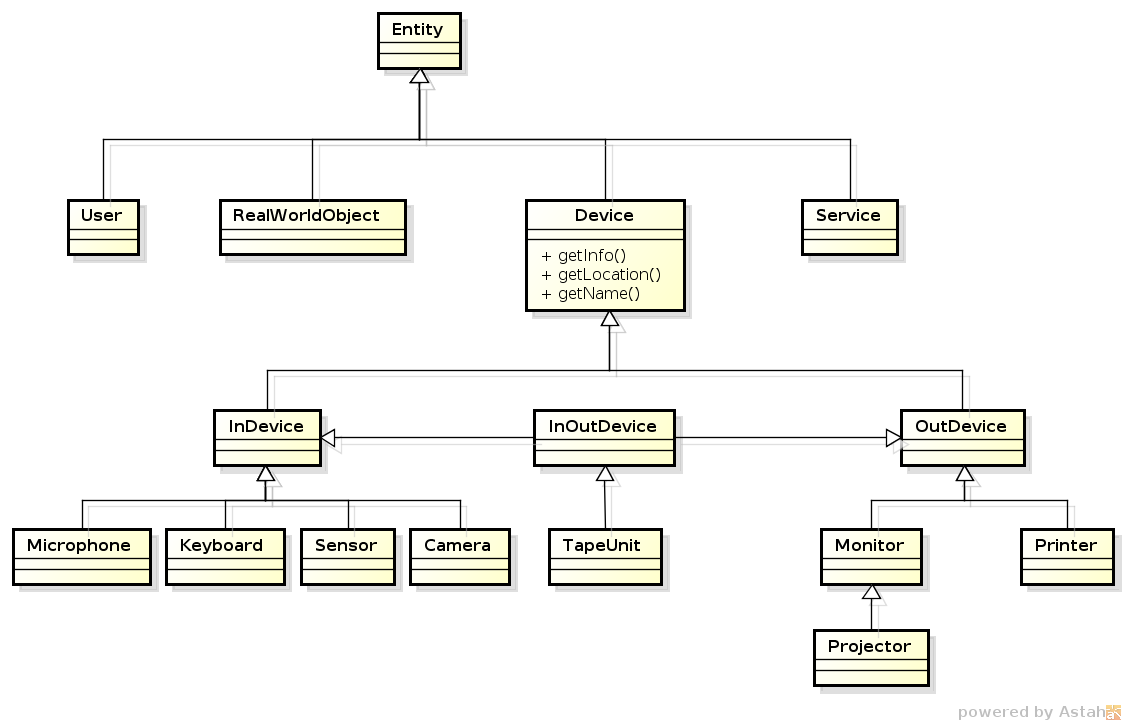
\includegraphics[scale=0.5]{imagens/gaia-devices}
\caption{Diagrama de Classes Simplificado~\cite{gaiaDevices}}
\label{fig:gaiaClassDiagram}
\end{figure}

No projeto, foi desenvolvido um \emph{framework} para a interação entre dispositivos heterogêneos. Esse \emph{framework} permite a representação das interfaces dos dispositivos com diferentes níveis de detalhe e especialização. As interfaces são definidas utlizando IDL(\emph{Interface Description Language}), que permite a construção de \emph{drivers} de dispositivos em qualquer linguagem de programação. 

A figura~\ref{fig:gaiaClassDiagram} mostra o Diagrama de Classes simplificado do projeto Gaia. Podemos observar que a Classe \emph{Device} é especializada em dispositivos de entrada(\emph{InDevice}) e saída(\emph{OutDevice}) de dados. Os dispositivos de entrada são ainda especializados em: Microfone, Câmera, Teclado e Sensor, enquanto os dispositivos de saída são especializados em: Impressora e Monitor, que por sua vez, é especializado em Projetor. Há ainda a interface para dispositivos que são de entrada e saída que é especializada em uma unidade de Fita.

\begin{comment}
http://gaia.cs.uiuc.edu/html/device.htm
http://gaia.cs.uiuc.edu/papers/GaiaSubmitted3.pdf
\end{comment}

\subsection{Amigo}
O projeto Amigo (\emph{Ambient Intelligence for the Networked home environment}) desenvolveu um \emph{middleware} com arquitetura baseada em SOA que integra dinamicamente sistemas heterogêneos para alcançar a interoperabilidade entre serviços e dispositivos. O middleware provê a semântica para comunicação e descoberta de dispositivos e serviços disponíveis no ambiente, incluindo dispositivos que utlizam padrões para descoberta como o UPnP integrando dispositivos móveis, computadores pessoais, eletrodomésticos e dispositivos de automação residencial~\cite{amigoArch}.

\begin{figure}[ht]
\center
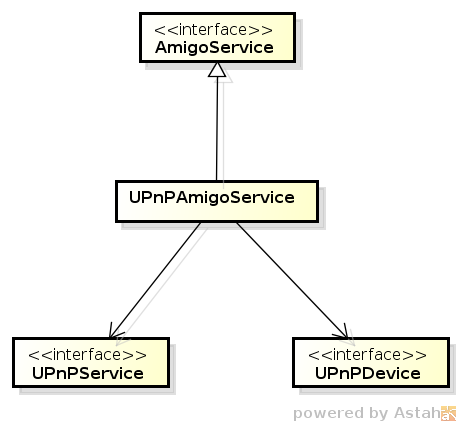
\includegraphics[scale=0.5]{imagens/amigo-interfaces}
\caption{Implementação de um \emph{AmigoService} utilizando serviços UPnP~\cite{amigoCore}}
\label{fig:amigoInterfaces}
\end{figure}

Além de utilizar o UPnP para a descoberta de dispositivos, o Amigo é compatível com as classificações de dispositivos do UPnP. Quando um dispositivo UPnP é encontrado, é criada uma instância de um \emph{UPnPDevice} e o \emph{driver AmigoUPnP} é notificado e executa o método \emph{getServices} do \emph{UPnPDevice} e cria para cada serviço uma instância do \emph{UPnPAmigoService}. A figura~\ref{fig:amigoInterfaces} mostra o relacionamento entre as interfaces UPnP com a implementação de uma interface de um Serviço do Amigo.

Os serviços do Amigo são modelados em uma Ontologia que é utilizada para comparar serviços e decidir se eles são equivalentes. A classe central da Ontologia é o Componente que representa o dispositivo provê o serviço. Para representar o que o dispositivo requer e provê, foi introduzido o conceito da Capacidade, dividida em Capacidade Requuerida e Capacidade Provida. Uma Capacidade possui parâmetros de entrada e saída que também são modelados em classes. As capacidades são então associdas à Conversas suportadas pelo Componente e relacionadas à mensagens que são empregadas na Conversa associada como mostra a figura ~\ref{fig:amigoServiceOntology}.

\begin{figure}[ht]
\center
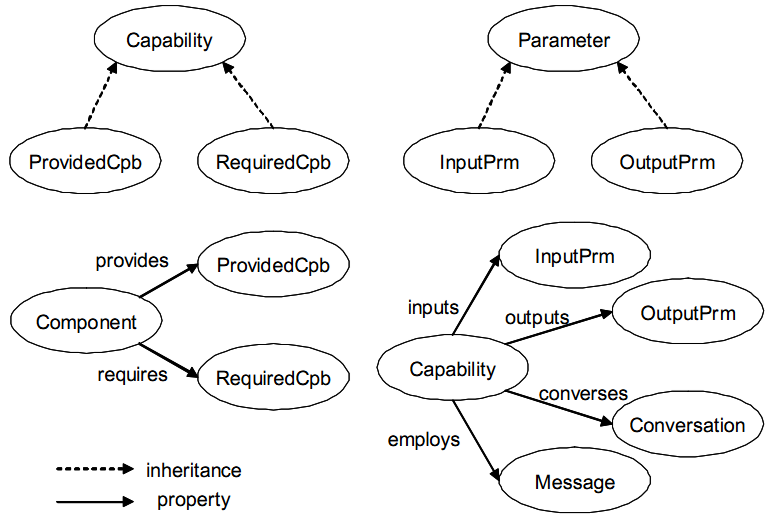
\includegraphics[scale=0.5]{imagens/amigo-ontology}
\caption{Elementos básicos da Ontologia de Serviços~\cite{amigoCore}}
\label{fig:amigoServiceOntology}
\end{figure}


\begin{comment}
http://www.hitech-projects.com/euprojects/amigo/publications/IST-004182%20Amigo-IP%20short%20project%20description.pdf
http://www.hitech-projects.com/euprojects/amigo/deliverables/Deliverable%20D1.2-VolII_SOTA_v10_final.pdf
http://www.hitech-projects.com/euprojects/amigo/deliverables/Amigo_WP2_D2.1_v10%20final.pdf
http://www.hitech-projects.com/euprojects/amigo/deliverables/Amigo_WP3_D31b_v1.0.pdf
\end{comment}

\subsection{\emph{Gator Tech}}

O projeto \emph{Gator Tech Smart House} é o resultado de mais de cinco anos de pesquisa na área de computação pervasiva e móvel. O objetivo do projeto é criar ambientes assistivos como casas que terão conhecimentos sobre si e sobre seus residentes criando um mapeamento entre o mundo físico, monitoramento remoto e serviços de intervenção~\cite{gatorTech}.

Neste projeto foi desenvolvida uma arquitetura para plataforma de sensores orientada à serviços, o Atlas. A plataforma Atlas é uma combinação de nós de \emph{hardware} e \emph{firmware} executado em um \emph{hardware} e um \emph{middleware} executando na rede, que provê serviços em um ambiente. Juntos, esses componentes permitem que qualquer sensor, atuador ou qualquer outro dispositivo sejam integrados e controlados por meio da interface de um determinado dispositivo. Essa abordagem facilita o desenvolvimento de aplicações que utilizam esses dispositivos~\cite{gatorTechLessons}. 

O Atlas é responsável por obter a representação de serviços dos dispositivos conectados e gerenciar os serviços de modo que as aplicações possam obter e utilizar os serviços facilmente. Na implementação do \emph{Gator Tech}, a camada de serviços foi construída sobre o \emph{framework} OSGi que matém o registro dos serviços de todos os nós conectados. Cada sensor ou atuador é representado no \emph{middleware} Atlas como um pacote de serviços OSGi. Inicialmente esses serviços eram representados em classes Java. Entretanto, a criação desses pacotes não acontecia de forma automática. 

\begin{figure}[ht]
\center
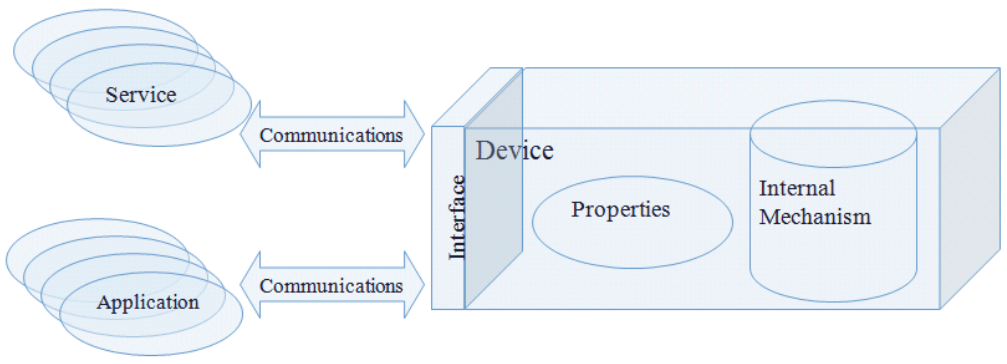
\includegraphics[scale=0.4]{imagens/gatorDDL}
\caption{Caracterização de um Dispositivo~\cite{ddlSpec}}
\label{fig:ddlspec}
\end{figure}

Para cada modelo de sensores e atuadores, era necessário ler a especificação do fabricante, examinar a interface e estudar os protoclos de comunicação. Era necessário ainda, que quem escrevesse o pacote fosse especialista na programação Java e no \emph{framework} OSGi. Com o objetivo de resolver essa complexidade o grupo de pesquisa do Atlas desenvolveu a \emph{Device Description Language}(DDL). Essa linguaguem provê um esquema capaz de descrever a interface dos dispositivos e um processador da linguagem para converter DDL para pacote de serviços OSGi que separa as responsabilidades entre fabricantes de dispositivos, integradores de sistemas e programadores de aplicativos~\cite{gatorTechDDL}.

Na DLL, um dispositivo é caracterizado como uma entidade com propriedades, mecanismo interno e uma interface. Como mostra a figura~\ref{fig:ddlspec}. As propriedades provêem informações a respeito do dispositivo com seu propósito, suas capacidades, fabricante e requisitos operacionais. Essas informações são críticas para a integração do sistema e para programadores de serviços. O mecanismo interno é responsável pela operação do dispositivo e é desconhecido do mundo externo. A interface do dispositivo é a ponte entre o hiato entre o mecanismo interno e o mundo externo. Ela especifica a entrada e saída do dispositivo e provê um guia para aplicações e outros serviços interagirem com o dispositivo.

Os dispositivos foram classificados em três categorias:
\begin{itemize}
	\item Sensor: apenas provê dados de entrada para o usuário externo.
	\item Atuador: apenas aceita dados de saída do usuário externo.
	\item Dispositivo Complexo: provê dados de entrada e aceita dados de saída do usuário externo.
\end{itemize}

Essa classificação genérica tem a disvantagem de ser difícil de ser reutilizada e especializada por diferentes dispositivos, sendo que seus recursos são expostos na forma de serviços por meio da especificação de operações~\cite{ddlSpec}.


\section{Comparativo}
%Apresentar um Comparativo entre as estratégias e conclusões que embasem a definição da proposição de vcs no capítulo seguinte.
Nesta seção faremos um comparativo dos padrões mostrados de forma a embasar a classificação de recursos que será proposta no próximo capítulo. 

\begin{table}
	\begin{center}
		\begin{tabular}{cllllll}
		\hline
						& \textbf{IEEE 1451} & \textbf{Bluetooth} & \textbf{USB} & \textbf{UPnP} & \textbf{DLNA} & \textbf{DDL}\\
		\hline
		\hline
		%Propósito 		& Permitir comunicação entre transdutores & Substituir os cabos de conexão mantendo altos níveis de segurança & Integrar interfaces existentes em uma única & Facilitar conectividade entre dispositivos & Partilha de conteúdo digital & Diminuir a complexidade na definição de um dispositivo \\
		\hline
		Classificação 	& Relacionada & Fixa & Relacionada & Relacionada & Relacionada & Fixa \\
		\hline
		Representação 	& IDL & & "Descritor de Dispositivo?" & XML & XML & XML \\ 
		\hline
		Extensível 		& Não & Não & Sim & Sim & "Não parece" & Não \\
		\hline
		Permite Múltiplas Classes & Sim & & Sim & Não & Sim & Não \\
		\hline
		Vantagem 		& & & & & & \\
		\hline
		%Desvantagem 	& & & & Necessária Homologação de novos dispositivos & & Por utilizar poucas categorias, dificulta a especialização de dispositivos\\
		\hline
		\end{tabular}
	\end{center}
	\caption{Comparativo dos Padrões.}
	\label{tab:comparativo}
\end{table}
 
%Como pôde ser observado, os padrões existentes para a classificação de recursos mostrados neste trabalho são todos estruturados, ou seja, não foi utilizada uma forma dinâmica como uma Ontologia para representar essa classificação.
